\documentclass{report}
\usepackage[utf8]{inputenc}
\usepackage[danish]{babel}
\usepackage{amsmath}
\usepackage{graphicx}
\usepackage{subfig}
\begin{document}
\setcounter{chapter}{0}

%Forside
\title{Projektarbejde, Snake}
\date{18. januar, 2015}
\author{	Anna Ølgaard Nielsen - 			s144437\\
Christian Søholm Andersen 	- s103080\\
Mathias Enggrob Boon - 			s144484\\
Van Anh Tri Trinh - 				s144449}

\maketitle

%Indholdfortegnelse
\tableofcontents
\newpage
\setcounter{chapter}{0}
%Første side
\pagenumbering{arabic}
\chapter{Introduktion}
Formålet med projektopgaven er at genskabe det klassiske spil "Snake", samt dokumentere hvordan spillet blev lavet.
Spillet er gengivet i to versioner: Simpel-snake og Avanceret Snake. Simpel-snake er en primitiv version af spillet, hvor styring kun foregår vha. input fra brugeren. I Avanceret Snake er der tilføjet forskellige funktioner, som enten forbedrer brugerfladen, f.eks. tilføjelse af hovedmenu, eller ændrer spillet, f.eks. automatisk bevægelse af slangen.
I rapporten vil designet af begge spillets versioner blive forklaret, samt implementationen af spillet. Kapitlet "Udviklingsproces" forklarer de tanker der ligger bag implementationen, og de valg der blev foretaget når der var flere mulige implementationer.

\begin{figure}[b]
	\centering
	\graphicspath{ {pics/} }
	\subfloat[Snake Menu]{\label{fig:menu}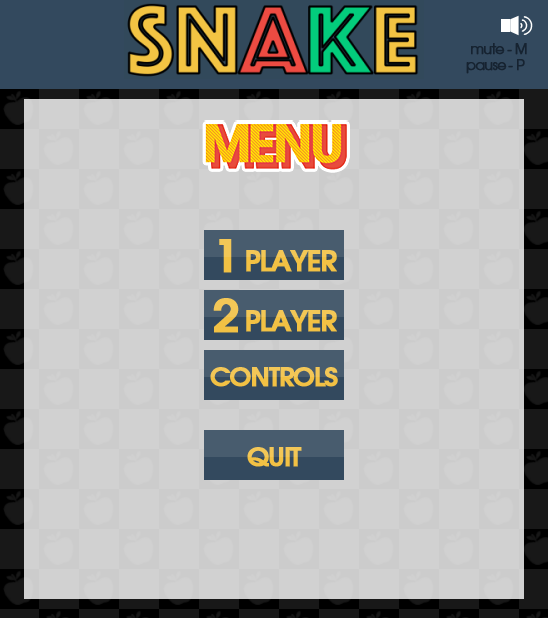
\includegraphics[width=0.3\textwidth]{snake.png}}
	\hspace{0.1\textwidth}
	\subfloat[Snake Game]{\label{fig:game}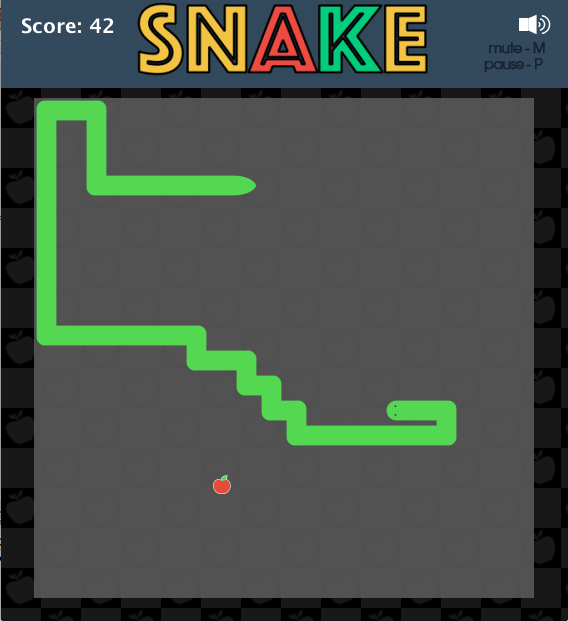
\includegraphics[width=0.31\textwidth]{snake2.png}}
\end{figure}

\chapter{Simple Snake}
\section{Afgrænsning}
I simpel-snake skal slangen bestå af to felter (et hovede og en hale), placeret i centrum af banen og rettet mod venstre. Det skal være muligt at bevæge sig frit på banen i de fire retninger vha. input fra tastaturet. Bevæger man sig udover banens kanter, skal man kunne fortsætte på den modsatte side. Det skal herudover være muligt  at øge slangens længde ved at bevæge sig over et felt med et "æble", og slutte spillet ved at bevæge sig ind i et felt udfyldt af slangen.
\linebreak

\section{Design}
Simpel-snake er designet, så selve spillet ligger i klassen Game. Game bruger da klasserne i model-pakken til at fylde spillet ud, f.eks. Board og Snake. Spillets tilstand ændres, når der modtages input fra control-klasserne, som bestemmer hvornår og hvordan slangen bevæger sig. I ??-klassen er en observer, som notificeres hver gang banens tilstand ændres. Når dette sker, samt når spillet startes, tegnes banen vha. klasserne View og BoardPanel. Disse klasser modtager information fra model-klasserne, f.eks. Snake, til at bestemme hvordan spillet skal gentegnes. BoardPanel gentegner hele spillet hver gang spillet opdateres. Først tegnes selve banen, derefter slangen og "maden". 
For at starte spillet bruges klassen Driver, som laver et nyt Game.
\linebreak

Snake-spillet er lavet efter et MVC-design, hvormed selve spillet, styringen af spillet og den visuelle repræsentation af spillet holdes adskilt i tre dele. På denne måde interagerer brugeren kun med den del af programmet, der er dedikeret til styring. Styringen manipulerer programmets tilstand i model-koden, som visualiseres i view-koden. Dette betyder derfor også, at alle funktioner, der påvirker programmets tilstand, skal holdes i model-koden. Control modtager kun input fra brugeren, og sender dette videre til view og eller model. View modtager input fra control og sender ændringerne i view videre til model. Det er derefter muligt at "observere" gennem en observer ændringerne i game, som bliver opdateret i view. 

\section{Implementering}


\subsection{Control (Styring)}
I simpel-snake bruges der kun 4 taster til input, nemlig de fire retningstaster, som derfor er defineret i control. Control-klassen har en metode, keyPressed, der kaldes hver gang der tastes. Hvis tasten er en af de fire retningstaster, kaldes funktionen moveSnake i Snake-klassen, med den tilsvarende retning som argument.

\subsection{Model}
Spillets model består af en række klasser, der tilsammen udgør selve spillet.
Klassen "Field" bruges til at definere et objekt, som kan opdele banen. Den fungerer på samme måde som Point-objekt-klassen, hvor koordinatsystemet starter oppe i venstre hjørne. Den eneste forskel mellem Point- og Field-klassen, er hvordan man kommer frem til et punkt. Point-klassen går først ud af x-aksen og derefter ned af y-aksen, hvorimod Field-klassen gør det omvendt. Da hele vores spilleplade er delt op i rows og column frem for x og y, er Field det optimale objekt at bruge.
\linebreak

Funktionenen equals er defineret i denne klasse, og bruges til at undersøge om to objekter ligger på samme felt, f.eks. slangens hoved og "æblet". Æblet er defineret i klassen "Food", hvor datafeltet "position" afgør dets nuværende position. 

Slangen selv er defineret i klassen "Snake". Slangens krop består af en række felter, hvoraf det første er hovedet, og de resterende er kroppen. Koordinaterne for disse felter er gemt som elementer i en LinkedList kaldet "positions". Det første element er slangens første led, hovedet, andet element er slangens andet led osv. Når et nyt led tilføjes, tilføjes et nyt element til listen. Dette bruges, når slangen spiser æblet. Som holder slangen stille, mens et nyt hovede tilføjes i den retning, man har trykket. 
Vi bruger linkedlist i stedet for arraylist, som vi startede med, fordi når man hver gang tilføjer et nyt hovede, så får hovedet den første plads, og alle andre elementer flyttes en gang tilbage. Når slangen er stor nok, kan dette godt komme til at lacke spillet lidt. Derfor er linkedlist helt klart mest optimalt at bruge, da den bare tilføjer et nyt element forrest uden at rykke alle de andre elementer.

Funktionen setupStartingSnake laver slangen ved at bestemme banens centrum, og tilføje to elementer til "positions" med centrumfeltet og feltet til venstre for dette felt.

Selve banen er defineret i Board-klassen, som har datafelterne height og width. Funktionen wrap undersøger om slangen er ved at bevæge sig ud over banens grænser. Er dette tilfældet, fortsætter slangen i stedet på den anden side af banen.

Når move-Funktionen kaldes, undersøges det først, om den nye retning er modsat slangens nuværende retning. Er dette tilfældet, sker intet. Er retningen gyldig, undersøges det om der ligger et æble på den nye plads. Hvis der gør, tilføjes et nyt element i ArrayListen "positions". 
Det undersøges næst, om slangen rammer sig selv, ved at sammenligne om det ønskede felt har samme koordinater som et af slangens led, undtagen halen. Er dette tilfældet, sættes spillets tilstand til LOST, hvormed spillet slutter. Hvis ikke, flytter slangen sin position, således at hovedet indtager et nyt felt, 2. led tager hovedets tidligere plads, 3. led tager 2. leds plads osv. Dette gøres ved, at ArrayListen opdateres bagfra, således at halen tager næstsidste leds koordinater, næstsidste led tager tredjesidste led osv. Når dette er gjort, tager hovedet den nye position, som afhænger af hvilket input der gives.

For at sikre, at maden altid placeres på et gyldigt felt, benyttes funktionen generateRandomFood i Food-klassen. Så længe slangen er under en hvis størrelse, placeres maden på et tilfældigt felt, hvorefter det sikres at feltet ikke er optaget af slangen. Er den det, placeres maden et nyt sted.

Er slangen større end $2*bredde*højde$, laves en ArrayListe over de felter, maden kan placeres på, hvorefter maden placeres tilfældigt på en af disse felter.

\subsection{View (Brugerflade)}
Brugerfladen er samlet i klassen View. View har en række funktioner, som sætter viser forskellige paneler. F.eks. bringer funktionen showGame spillebanen samt scorepanelet frem. 

\section{Udviklingsproces}
\subsection{Arbejdsproces}
Formålet med projektet var at starte med at lave en simpel udgave af snake, og derefter tilføje flere funktioner til at lave en mere avanceret version. Dette gør det ideelt at tilføje en funktion af gangen, hvormed programmet starter ud simpelt, men fungerende, hvorefter yderligere funktioner kan tilføjes. Programmet er altså udviklet iterativt, hvormed der opstår flere fungerende versioner af spillet, men med forskellige funktioner. Dette gør det muligt at tilpasse programmet, hvis der opstår ideer undervejs. 

Den iterative tilgang gør det muligt at have en "cyklus" for udviklingen af programmet. Først bestemmes det, hvad der skal tilføjes til programmet. Herefter kan opgaverne blive fordelt blandt gruppens medlemmer. Gruppemedlemmet afgør selv, hvordan en funktion skal designes og implementeres. Når en ny tilføjelse til programmet er færdig, testes den. Eventuelle justering til programmet laves for at undgå fejl med den nye funktion, hvorefter "cyklussen" starter forfra ved

\subsection{Controller}
	
\subsection{Model}

\subsubsection{Opbygning af banen}
Til designet af selve banen, som slangen bevæger sig på, forelå to muligheder. Den ene var at lave et to-dimensionelt array af datatypen enum, hvis størrelse afgør banens endelige størrelse. Et array [10][5] vil f.eks. give en bane med længden 10 og bredden 5. Hvert element i arrayet bestemmer da, hvad der befiner sig på netop denne plads på banen. Elementerne i arrayet kan f.eks. være et blankt felt, et æble, et led af slangen osv. Dette gør det nemt at introducere nye spilelementer i fremtiden, f.eks. bonus-point, vægge og miner, idet der blot skal tilføjes nye værdityper. Visualisering af spillet foregår ved at definere et billede for hvert spilelement, og få programmet til at tegne objektet på arrayets plads.
ULEMPER - observer?

En anden metode er, at lade de forskellige spilelementer være defineret i deres egne klasser, så f.eks. SnakeFood er en klasse for sig selv, SnakePlayer er en klasse for sig selv osv. Hver klasse har de funktioner, der er relevante for dem, f.eks. getPosition for at give deres nuværende position. Programmet tegner da spillet hver gang en tur afsluttes, dvs. når alle elementer som skal ændres, er ændret. Programmet har fået defineret billedet for de forskellige elementer, og modtager deres position vha. en getPosition metode.
 Ulempen ved denne metode er, at tegning af programmet gøres mere kompliceret. I den første metode er alle felter allerede defineret, og for at ændre dem behøves det blot at ændre værdien. Ønskes et spilelement ændret eller introduceret med den anden metode, skal der laves et nyt element.
 
Den anden metode blev valgt til spillet, idet det blev bestemt at den passede bedre til MVC-modellen, hvormed view-koden kun bruger de forskellige klassers get-metoder til at få information. %bum bum

\subsubsection{Snake}
Da slangen i snake-spillet består af en række felter, som alle har netop en koordinat i forbindelse med de resterende, er en effektiv måde at bestemme slangens position på en LinkedList, idet denne datastrukturer er fleksibel i størrelse og passer til formålet. Når slangen vokser i størrelse, bliver dette dog mindre effektivt, idet slangens hoved altid er element 0. Når slangen vokser, tilføjes et nyt element på plads 0, hvormed hele listen skal flyttes. En anden mulighed ville være at bruge en anden datastruktur, f.eks. LinkedList, eller lade hovedet være defineret som element positions.size()-1, hvormed nye hovedet tilføjes sidst i listen.

For at implementere scoren blev der fremlagt to løsninger. Enten at lade scoren være et datafelt i game-klassen, eller at lade det være en klasse for sig selv. Ved at lade scoren være et datafelt, bliver implementationen simplere. At lade scoren være en klasse for sig selv har derimod fordelen, at der kan 
tilføjes en observer til Score-klassen, som dermed kun opdateres, når scoren ændrer sig. Scorepanelet optegnes ikke i samme klasse som banen, og kan derfor holdes seperat, så scorepanelet kun gentegnes, når scoren ændrer sig. Hvis scoren derimod er et datafelt, tegnes scoren efter hver tur, også selvom scoren er uændret. I sidste ende blev det bestemt at holde scoren som datafelt, hvormed det også bliver simplere at implementere nye score-relaterede funktioner i fremtidige udgaver.

\subsection{Brugerflade og visualisering af programmet}
\subsubsection{Tegning af banen}


\subsubsection{Vinduestørrelse}
Området, som spillet foregår på, skal kunne bestemmes til at være mellem 5x5 og 100x100. Dette kan dog skabe problemer, hvis størrelsen bliver for stor, idet banen både skal være synlig, men også passe på en gennemsnitlig computerskærm. En bane på 10x10 kan sagtens passe på en opløsning af f.eks. 400x400, men øges banens størrelse til 50x50, bliver banen svær at se. Herudover varierer skærmstørrelser, og det er derfor nødvendigt at gøre spillets vinduestørrelse fleksibel. En løsning på dette problem ville være at bestemme en fast størrelse for felterne, og lade vinduet justere sin størrelse efter dette. Ønskes det f.eks. at felterne altid har størrelsen 20x20, og at banen skal være 15x25, vil vinduets størrelse blive 300x500. Fordelen ved denne metode er at det sikres, at banen altid er synlig, og at der ikke opstår problemer, fordi forholdet mellem vinduets størrelse og banen størrelse ikke passer sammen. Ulempen ved metoden er, at store baner kan blive for store til at være på en normal skærm. F.eks. vil en bane med felter af størrelsen 20x20 og banestørrelsen 75x75 fylde 1500x1500. Herudover er løsningen ikke brugervenlig, idet en bruger kan blive forvirret over hvorfor vinduets størrelse ændrer sig fra bane til bane, og måske ligefrem ikke passer på skærmen.

En anden metode er at gøre vinduet justerbart. Denne løsning er mere brugervenlig, idet vinduets størrelse frit kan justeres så det passer til den enkelte person. Denne metode introducerer dog et andet problem, nemlig at felternes størrelse skal skaleres til at passe vinduet. Nogle opløsninger af vinduet vil ikke være et multiplum af banens størrelse, hvormed elementerne i spillet vil blive aflange. Dette problem blev løst ved at lave en baggrund og låse banens forhold, hvormed banen altid fylder mest muligt af vinduet ud, og den resterende plads bliver udfyldt af baggrunden. Idet denne løsning var mere nemmere at bruge og forstå, og giver bedre mulighed for justering af spillet, blev den valgt i stedet for løsning 1.

\section{Evaluering}
-To eller en Arraylist -> linklist ?
-Point -> Field
-Int -> Enum (direction)
-width+height <-> kvadratisk variabel ?
-Banens opbygning: double-array -> positions-placering
-Optimering af runtime i “food”-klassen (dobbelt for-loop eller random placering)
-brug af observer - får model-view-controller til at gå op
-Flere opgaver er givet til “game”-klassen frem for de andre klasser

\chapter{Avanceret Snake}
\section{Afgrænsning}
I den avanceret del har vi valgt at lave spillet, som hvis det var et hvilket som helst professionelt snake-spil, man kan finde på nettet. Derfor er der lagt fokus på grafikken af spillet inklusiv menu'en, og på alle de små shortcuts og valgmuligheder, der er i et almindeligt simpelt computerspil. Derudover har vi ændret kravet for slangens bevægelse til, at den bevæger sig ved hjælp af en timer som en slags animation. Vi har dog beholdt simple-snake som en "kindergarten"-sværhedsgrad, som man kan vælge i menu'en.
På den måde har vi prioriteret de elementer, som "burde" være implementeret i et almindeligt computerspil. 

-----Skriv om multiplayer + evt. netværk---------
\section{Design}

\section{Implementering}

\subsection{Control (Styring)}
Derudover er der også implementeret en masse shortcuts, som nemt styrer en igennem menu'en og giver ekstra funtioner i spillet. Fra keyboarded er der blevet implementeret følgende shortcuts: Mute-button (M), pause-button (P), menu-button (Esc), tilbage-button (Back-Space), (re)start-button (enter/space), som (gen)starter spillet i default-mode.
Gennem JButton er der også blevet implementeret en masse knapper i menu'en, game-over-mode, og restart-mode, som er styret af musen i ActionListener.

Der er lavet en controller-klasse for hver menu-side og en for spillet (ControlBoard), derudover har vi en control-klasse, der skal gælde for både menu'en og spillet, heri ligger både mute-funktionen og tilbage-til-menu'en-funktionen.

\subsection{Model}

\subsection{View (Brugerflade)}
----Selv lavet logo, slange, æble, knapper, baggrund og alle andre billeder selv - intet fra nettet (uden audio)----
-color (dobbelt for-loop - pixels)


\section{Udviklingsproces}

\subsection{Optegnelse af slange}

I simpel-snake kan spilleren se hvor han har været, men ikke i hvilken rækkefølge. Spilkvaliteten kunne dermed forbedres, ved at lade spilleren se, hvordan slangen har bevæget sig. Det ønskede resultat ville være, at hvert af slangens led er forbundet med det forrige og næste, og så har fri plads i de områder, der ikke er forbundet.
For at opnå dette blev der lavet en ny klasse, Bodytype, til at definere hvordan slangens led skal se ud. I snake-klassen blev en ny ArrayList tilføjet, nemlig body, som bruges til at bestemme Bodytype for de forskellige led. Bodytype(0) er dermed hovedet, bodytype(1) er første led osv. Hver bodytype består af to datafelter af typen "relation", hvis værdi er afgjort af det forrige og næste led. Er det forrige led f.eks. over det nuværende, er prev = ABOVE. Er det næste led til højre for det nuværende led, er next = BESIDERIGHT.
Leddenes Bodytype skal naturligvis opdateres efter hver tur. Dette gøres af funktionen updateBody, som vha. en for-løkke går gennem alle elementerne. Det undersøges da, om positionen for det forrige og næste led er over, under, til højre eller venstre for det nuværende led, og prev samt next sættes til at passe dette. updateBody kaldes hver gang slangen bevæger sig.

\subsection{Lyd}

Som en mindre tilføjelse til spillet er lyd tilføjet i form af Audio-klassen. Funktionerne i Audio-klassen bruget til individuelt at spille 	

\subsection{Menu}

\subsection{Automatisk bevægelse}
-----Husk at skriv noget om incrementet timer-------

\subsection{Multiplayer}

\section{Evaluering}
-ingen brug af jbutton -> jbutton
-Se alle slangens led - gør den lidt forsinket, når den er lang



\chapter{Konklusion}

\end{document}

